\section{Finding 3 - Exact Apache Version can be determined}
%center under chapter title a one row table with 6 coloumns and no borders
\vspace*{-0,3cm}
\begin{center}
    \begin{tabular}{c c c c}
        \textbf{Classification:} & Information Disclosure & \textbf{Severity:} & \textbf{\textcolor{green!50!blue}{Low}}  
        \end{tabular}
\end{center}

\vspace*{-0,8cm}
\begin{center}
    \begin{tabular}{c c}
        \textbf{CVE:} & Null
    \end{tabular}
\end{center}

Visiting port 80 of the \ac{DUT} in a web browser with the path ”/home” reveals the exact version of Apache that is running on the \ac{DUT}.  The version of Apache that is running on the \ac{DUT} is \textbf{”Apache/2.4.54 (Debian)”}. This Finding has a low severity, because it should be more important to use a newer version of Apache to prevent exploits of known vulnerabilities.


\subsection{Finding Impact}
This can be used to find known vulnerabilities in the version of Apache that is running on the \ac{DUT}. These vulnerabilities can be found in chapter 4.

\subsection{Finding Details}
%insert an image of the webbrowser
\begin{figure}[h]
    \centering
    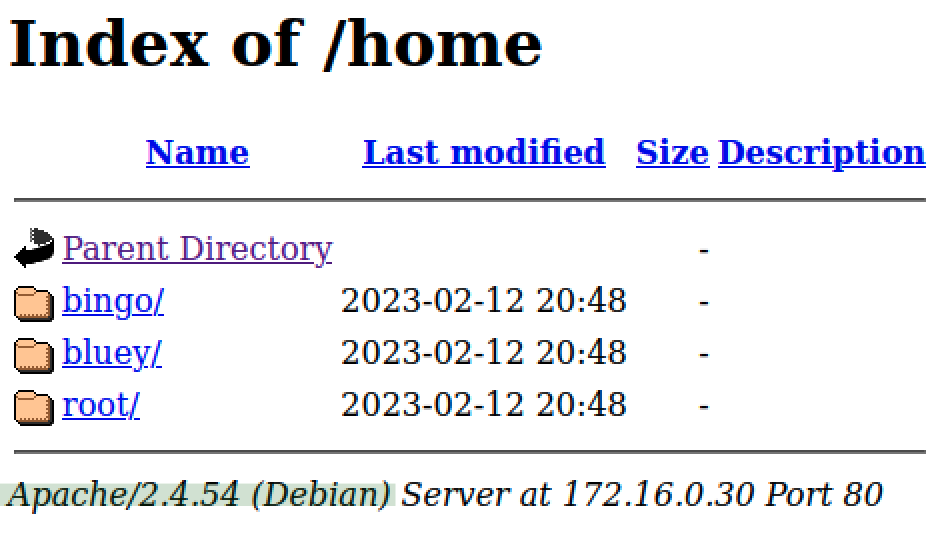
\includegraphics[width=0.8\textwidth]{img/apache-version.png}
    \caption{Apache Version}
    \label{fig:fin3}
\end{figure}

\subsection{Evaluation of Results}
\begin{center}
    \begin{tabular}{cccc}
    \textbf{Effort to Fix:} & &\ \textbf{\textcolor{orange}{Medium}}\
    \end{tabular}
\end{center}
How do you judge the individual technical findings (severity, likelihood)?
What is your suggested remediation, if there is one?
How can the customer validate their remediation is effective once implemented?